\documentclass[12pt, utf8, hyperref]{article}
\usepackage{ctex}
\usepackage{graphicx}
\usepackage{float}
\usepackage{amsmath}
\usepackage{listings}
\usepackage{xcolor}
\usepackage{lipsum}

\hypersetup{
    colorlinks=true,
    linkcolor=black
} %set link in table of contents to black (default red)

\definecolor{vgreen}{RGB}{104,180,104}
\definecolor{vblue}{RGB}{49,49,255}
\definecolor{vorange}{RGB}{255,143,102}
\lstset
{
    backgroundcolor=\color[RGB]{245,245,244},
    basicstyle={\footnotesize\ttfamily},        % set code style
    keywordstyle=\color{vblue},
    identifierstyle=\color{black},
    commentstyle=\color{vgreen},
    % numbers=left,                      % set line numbers
    numberstyle={\tiny \color{black}}, % set fonts of line numbers
    frame=lines,                      % set type of open 
    numbersep=10pt,
    breaklines=true,                   % automatic line break
    tabsize=4,
    aboveskip=10pt,
    belowskip=2pt
}
% \setlength\parindent{0pt} %default no indent

\begin{document}
\begin{titlepage}

% 首行的位置往上调整。但vspace前面需要有东西才会起效。
\begin{figure}[H]
	\centering
	
\includegraphics[scale=0.5]{photos/logo.png}
\end{figure}

\phantom{Start!}
\vspace{1.7cm}
\begin{center}

% Title
{ \Huge \bfseries An interesting Course}\\[0.4cm]
{ \huge \bfseries Report of lab1}
\end{center}

\vfill

\begin{center}
{
% \pillar:使用一种统一的方法提高行高
\newcommand{\pillar}{ {\Huge \phantom{A}} }
\large
\begin{tabular}{lc}
\pillar 姓名 & Clarence Wang \\\cline{2-2}
\pillar 学号 & 2016011111 \\\cline{2-2}
\pillar 班级 & Your class \\\cline{2-2}
\pillar 实验日期 & \today \\\cline{2-2}
\pillar 报告日期 & \today \\\cline{2-2}
\end{tabular}
}
\end{center}
\end{titlepage}
 
\section{First Section}
\lipsum[5]
\[
    f(x+h) = f(x)+hf'(x)+\frac{{h}^{2}}{2}f''(\xi) \quad \xi \in [x, x+h]
\]

\section{Second section}
\lipsum[5]
\begin{lstlisting}[language=matlab]
    sum=0;
    i=1;
    while(1/i/sum>0.5*6*10^(-8))
        sum=sum+1/i;
        i=i+1; 
    end
    disp(i);
\end{lstlisting}

\lipsum[4]
\begin{figure}[H]
	\centering
	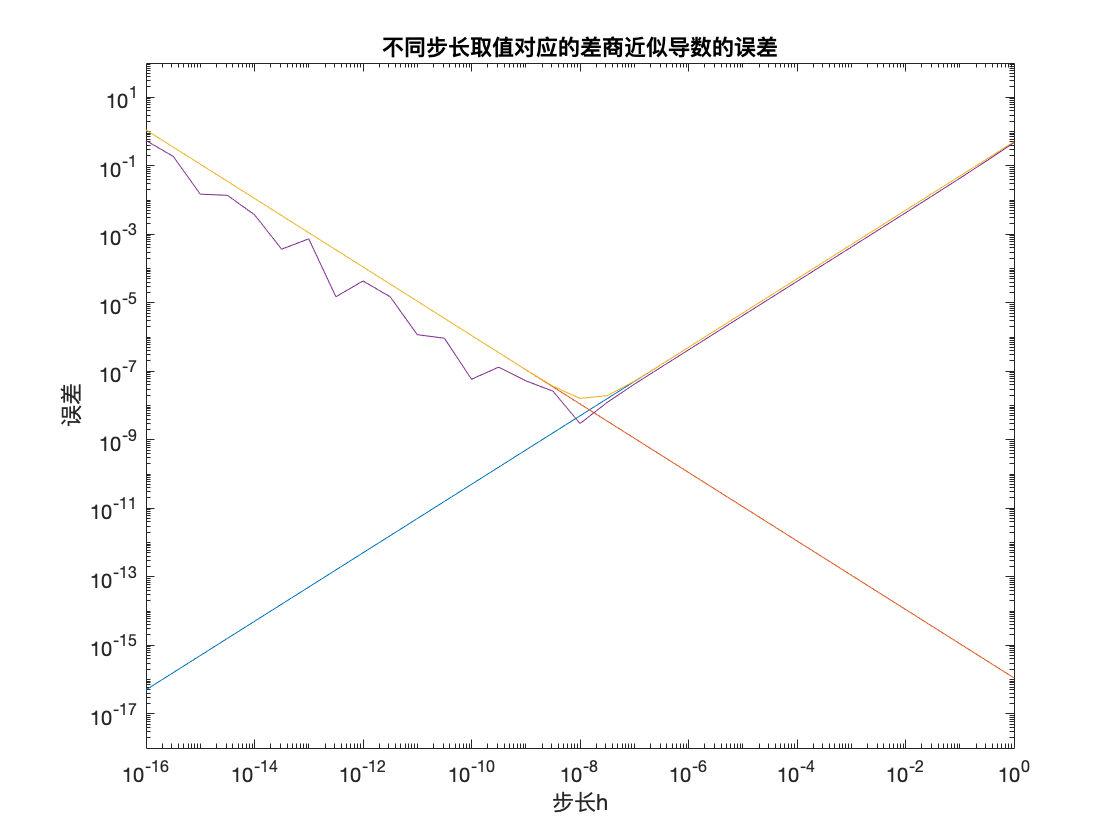
\includegraphics[scale=0.3]{photos/fig.png}
\end{figure}

\end{document}
